% Provenance (never printed): see sources/outline_sources.md (Year 3:
% geophysical fluid dynamics: rotating-frame equations, Rossby number,
% hydrostatic and geostrophic balance, thermal wind, buoyancy frequency).
% Brief: sources/book5/BRIEFS.md, ch. 19. Curves from
% figdata/bachelor-3/inertial_oscillation.py, thermal_wind.py and
% buoyancy_frequency.py. Exercise and problem values in the Book 5 scratch
% calculator calc/ch19.py. The Steppe of Orrin, its lake, its stations and
% its winds are invented.
\chapter{Dinámica de fluidos geofísicos}\label{ch:b3:gfd-foundations}

Al remover una taza de té, el remolino se apaga en un minuto; las hojas se
concentran en el centro del fondo y no ocurre nada más. El océano y la
atmósfera también se agitan, por el Sol y por el viento, pero en un planeta
que rota y en capas de distinta densidad. La rotación y la estratificación
las obligan a obedecer reglas que una taza de té nunca muestra: los vientos
soplan a lo largo de las isobaras y no a través de ellas, las columnas de
fluido se niegan a inclinarse y el viento de la alta troposfera queda
escrito en las temperaturas de abajo. Este capítulo plantea las ecuaciones
de estos flujos grandes, lentos y delgados, y los pocos números que deciden qué términos importan.

\begin{recall}
Las fuerzas de Coriolis y centrífuga en un sistema de referencia en rotación, las ecuaciones de Navier--Stokes
y de continuidad, la viscosidad, el número de Reynolds y la relación hidrostática
están en los libros de física. El parámetro de Coriolis $f = 2\Omega
\sin\varphi$, la fuerza del gradiente de presión, el equilibrio geostrófico, los
vientos geostrófico y del gradiente y las corrientes en chorro están en el
volumen de primer año, en su capítulo sobre la circulación general de la atmósfera; la
capa de Ekman en su capítulo sobre la circulación del océano; la temperatura
potencial, la estabilidad estática y la oscilación de una partícula de aire
elevada, en su capítulo sobre la estructura de la atmósfera y del océano.
\end{recall}

\section{Ecuaciones en un sistema de referencia en rotación}\label{sec:b3:gfd-foundations:equations}

En un sistema de referencia que gira con la Tierra a la velocidad angular
$\vec\Omega$, una partícula de fluido de velocidad $\vec u$ cumple
\[
\frac{\mathrm D\vec u}{\mathrm Dt} + 2\vec\Omega\times\vec u =
-\frac{1}{\rho}\nabla p + \vec g + \nu\nabla^2\vec u ,
\qquad
\frac{\partial\rho}{\partial t} + \nabla\cdot(\rho\vec u) = 0 ,
\]
donde $\mathrm D/\mathrm Dt = \partial/\partial t + \vec u\cdot\nabla$ es
la derivada siguiendo la partícula y $\nu$ la viscosidad cinemática. La
fuerza centrífuga se ha sumado a la gravitación: su suma $\vec g$ es la
gravedad efectiva, normal a las superficies de nivel del \omterm{def:b3:gravity-geodesy:geopotential}{geopotencial}, y la
vertical se define por ella. De la rotación solo queda el término de Coriolis, $-2\vec\Omega\times
\vec u$, que no realiza trabajo: hace girar una partícula
sin cambiar su rapidez. La Tierra gira a $\Omega =
\qty{7.292115e-5}{rad/s}$, con un día sideral de \qty{23.9345}{h}.
% ledger: geod5:grs80-defining, earth:Trot

Para movimientos a distancias mucho menores que el radio terrestre $a$, basta
con un sistema cartesiano local: $x$ hacia el este, $y$ hacia el norte, $z$
hacia arriba, a la latitud $\varphi$, en el plano tangente de la figura de abajo. Allí
$\vec\Omega = \Omega\,(0, \cos\varphi, \sin\varphi)$, y las tres
componentes de la ecuación de cantidad de movimiento son
\[
\begin{aligned}
\frac{\mathrm Du}{\mathrm Dt} - f v + \tilde f w &= -\frac{1}{\rho}\frac{\partial p}{\partial x} + F_x ,\\
\frac{\mathrm Dv}{\mathrm Dt} + f u &= -\frac{1}{\rho}\frac{\partial p}{\partial y} + F_y ,\\
\frac{\mathrm Dw}{\mathrm Dt} - \tilde f u &= -\frac{1}{\rho}\frac{\partial p}{\partial z} - g + F_z ,
\end{aligned}
\qquad f = 2\Omega\sin\varphi,\quad \tilde f = 2\Omega\cos\varphi ,
\]
con $\vec F$ la fricción. Para los flujos delgados y casi horizontales del
océano y de la atmósfera se desprecian los términos en $\tilde f$: $\tilde f w$
es pequeño frente a $fv$ porque $w \ll v$, y $\tilde f u$ es una diezmilésima
parte de $g$ (véase el \cref{exo:b3:gfd-foundations:5}). La fuerza de Coriolis actúa solo
en la horizontal, a través de la componente vertical local de
la rotación, $\Omega\sin\varphi$.

\begin{definition}[Plano $f$ y plano $\beta$]\label{def:b3:gfd-foundations:planes}
Cerca de una latitud de referencia $\varphi_0$, la aproximación del \emph{plano $f$}\index{plano f@plano $f$}
toma el parámetro de Coriolis como constante, $f = f_0 =
2\Omega\sin\varphi_0$. La aproximación del \emph{plano $\beta$}\index{plano beta@plano $\beta$}
conserva su variación de primer orden con la distancia hacia el norte $y$:
$f = f_0 + \beta y$, con $\beta = \mathrm df/\mathrm dy = 2\Omega
\cos\varphi_0/a$.
\end{definition}

A \ang{45}, con el radio medio $a = \qty{6371}{km}$, $f_0 =
\qty{1.031e-4}{s^{-1}}$ y $\beta = \qty{1.62e-11}{m^{-1}.s^{-1}}$: a lo largo de
\qty{1000}{km} de latitud $f$ cambia un \qty{16}{\percent}. El plano $f$
sirve para movimientos mucho menores que eso; el plano $\beta$ es necesario para
corrientes de escala de cuenca y ondas planetarias.
% ledger: earth:Rmean, geod5:grs80-defining (values in figdata/bachelor-3/inertial_oscillation.py)

\begin{omfigure}
\begin{minipage}[c]{0.42\linewidth}\centering
\begin{tikzpicture}[>=stealth, font=\small]
\draw[thick] (0,0) circle (2);
\draw[black!40, dashed] (-2,0) -- (2,0);
\draw[->, thick] (0,-2.4) -- (0,2.75) node[above] {$\vec\Omega$};
\draw (0,0) -- (30:2) coordinate (P);
\draw (0.6,0) arc (0:30:0.6);
\node at (15:0.9) {$\varphi$};
\draw[black!60] ($(P)+(120:-1.1)$) -- ($(P)+(120:1.3)$);
\draw[->, omThm, thick] (P) -- ++(0,1.6) node[right] {$\vec\Omega$};
\draw[->, omDef, thick] (P) -- ++(30:0.8) node[anchor=south west, align=left, inner sep=1pt] {$\Omega\sin\varphi$,\\ arriba};
\draw[->, omMeth, thick] (P) -- ++(120:1.386) node[anchor=south, align=center, inner sep=1pt] {$\Omega\cos\varphi$,\\ norte};
\draw[black!50, densely dotted] ($(P)+(30:0.8)$) -- ($(P)+(0,1.6)$) -- ($(P)+(120:1.386)$);
\draw (P) circle (0.09); \draw ($(P)+(-0.064,-0.064)$) -- ($(P)+(0.064,0.064)$);
\draw ($(P)+(-0.064,0.064)$) -- ($(P)+(0.064,-0.064)$);
\node[font=\scriptsize, anchor=west] at ($(P)+(0.14,-0.03)$) {$x$, este};
\node[font=\scriptsize, black!60] at (-1.15,-0.25) {ecuador};
\end{tikzpicture}
\end{minipage}\hfill
\begin{minipage}[c]{0.55\linewidth}\centering
\begin{tikzpicture}
\begin{axis}[width=\linewidth, height=0.72\linewidth, xmin=0, xmax=90, ymin=0, ymax=1.8,
  xlabel={latitud (\unit{\degree})}, ylabel={$f$ ($10^{-4}$\,\unit{s^{-1}})},
  xtick={0,15,30,45,60,75,90}, tick label style={font=\scriptsize}, label style={font=\small},
  legend style={font=\scriptsize, draw=none, fill=none}, legend pos=north west]
% computed in figdata/bachelor-3/inertial_oscillation.py
\addplot[omDef, thick] table[x=lat, y=f] {figdata/out/bachelor-3-inertial_oscillation-fbeta.dat};
\addplot[omThm, densely dashed] table[x=lat, y=fb] {figdata/out/bachelor-3-inertial_oscillation-fbeta.dat};
\addplot[only marks, mark=*, mark size=1.6pt] coordinates {(45,1.03126)};
\legend{$2\Omega\sin\varphi$, plano $\beta$ a \ang{45}}
\end{axis}
\end{tikzpicture}
\end{minipage}

\par\smallskip{\small A la izquierda, el marco local en la latitud $\varphi$: $z$
a lo largo de la vertical local, $y$ hacia el norte en el plano tangente, $x$ hacia el este
hacia dentro de la página. El vector de rotación se descompone en $\Omega\sin\varphi$ alrededor de la
vertical, que hace girar el movimiento horizontal, y $\Omega\cos\varphi$ alrededor del
eje hacia el norte, que se desprecia en flujos delgados. A la derecha, el parámetro de Coriolis y
su plano $\beta$ tangente en \ang{45}: cercano a él en una franja de latitudes,
y alejado de él cerca del ecuador y del polo.}\label{fig:b3:gfd-foundations:frame}
\end{omfigure}
% ledger: geod5:grs80-defining, earth:Rmean

Dos aproximaciones más simplifican las ecuaciones sin
perder lo que importa. La primera concierne a la densidad.

\begin{definition}[Aproximación de Boussinesq]\label{def:b3:gfd-foundations:boussinesq}
La \emph{aproximación de Boussinesq}\index{aproximación de Boussinesq} escribe
la densidad como $\rho = \rho_0 + \rho'$, con $\rho_0$ constante y
$|\rho'| \ll \rho_0$, y conserva $\rho'$ solo donde aparece multiplicada por $g$.
La ecuación de continuidad queda $\nabla\cdot\vec u = 0$, y la
ecuación de cantidad de movimiento
\[
\frac{\mathrm D\vec u}{\mathrm Dt} + f\,\vec k\times\vec u =
-\frac{1}{\rho_0}\nabla p' + b\,\vec k + \nu\nabla^2\vec u ,
\qquad b = -g\,\frac{\rho'}{\rho_0} ,
\]
donde $p'$ es la desviación de la presión respecto de la presión hidrostática
de la densidad $\rho_0$, $\vec k$ el vector unitario hacia arriba y $b$ la
flotabilidad.
\end{definition}

En el océano $\rho'$ es de unos \unit{kg/m^3} sobre \num{1025}, una fracción de un
por ciento, y la aproximación es excelente. En la atmósfera la densidad
disminuye en un factor $e$ en unos \qty{8.5}{km}; la aproximación se cumple para
capas mucho más delgadas que eso, y los flujos más profundos sustituyen $\rho_0$ por un
perfil medio $\rho_0(z)$, con la misma física.
% ledger: earth:Hscale

La segunda concierne a la vertical. Un fluido en reposo está en equilibrio
hidrostático; un fluido en movimiento lo mantiene con muy buena aproximación cuando
el movimiento es mucho más ancho que profundo.

\begin{definition}[Aproximación hidrostática]\label{def:b3:gfd-foundations:hydrostatic}
La \emph{aproximación hidrostática}\index{aproximación hidrostática}
sustituye la ecuación de cantidad de movimiento vertical de un fluido en
movimiento por la relación hidrostática, $\partial p/\partial z = -\rho g$.
\end{definition}

\begin{proposition}[Cuándo se cumple la aproximación hidrostática]\label{prop:b3:gfd-foundations:hydrostatic}
Para un movimiento de escala horizontal $L$, profundidad $H$ y velocidad $U$, con un
\omterm{def:b3:gfd-foundations:numbers}{número de Rossby} $U/(fL)$ como máximo de orden uno, la aceleración vertical es
menor que el gradiente vertical de la perturbación de presión en un factor
de orden $(U/fL)\,(H/L)^2$.
\end{proposition}

\begin{proof}
Cuando la fuerza de Coriolis es al menos tan grande como la aceleración, la
ecuación de cantidad de movimiento horizontal equilibra el gradiente horizontal de presión
con ella: $p'/(\rho_0 L) \sim fU$, luego $p'/\rho_0 \sim fUL$, y el
gradiente vertical es $p'/(\rho_0 H) \sim fUL/H$. La continuidad, $\partial w/\partial z
= -(\partial u/\partial x + \partial v/\partial y)$, acota la velocidad vertical
por $W \sim UH/L$, y la aceleración vertical por
$\mathrm Dw/\mathrm Dt \sim UW/L = U^2H/L^2$. El cociente es $(U^2H/L^2)/(fUL/H)
= (U/fL)(H/L)^2$.
\end{proof}

Un sistema meteorológico de \qty{1000}{km} de ancho en una troposfera de \qty{10}{km} de profundidad tiene
$(H/L)^2 = 10^{-4}$ y un \omterm{def:b3:gfd-foundations:numbers}{número de Rossby} de unos 0.1: el error de la
\omterm{def:b3:gfd-foundations:hydrostatic}{aproximación hidrostática} es del orden de $10^{-5}$. Falla solo en movimientos estrechos y profundos: una
corriente ascendente de tormenta, una pluma convectiva en el océano.

\section{Escalas del flujo en rotación}\label{sec:b3:gfd-foundations:scales}

Qué términos de la ecuación de cantidad de movimiento importan lo deciden dos cocientes.

\begin{definition}[Números de Rossby y Ekman]\label{def:b3:gfd-foundations:numbers}
Para un flujo de velocidad $U$, escala horizontal $L$ y profundidad $H$ sobre un planeta de
parámetro de Coriolis $f$, el \emph{número de Rossby}\index{número de Rossby} es
$\mathrm{Ro} = U/(fL)$, el cociente entre la aceleración, de orden $U^2/L$,
frente a la fuerza de Coriolis, de orden $fU$. El \emph{número de
Ekman}\index{número de Ekman} es $\mathrm{Ek} = \nu/(fH^2)$, el cociente entre
la fuerza viscosa, de orden $\nu U/H^2$, y la fuerza de Coriolis; en un
flujo turbulento $\nu$ se sustituye por una viscosidad de remolino.
\end{definition}

Un desagüe de bañera que evacua \qty{0.1}{m/s} sobre \qty{0.3}{m} tiene un \omterm{def:b3:gfd-foundations:numbers}{número de Rossby} de
algunos miles: la rotación terrestre no decide el sentido de su remolino. Una depresión de
\qty{1000}{km} de diámetro con vientos de \qty{15}{m/s} tiene
$\mathrm{Ro} \approx 0.14$, y un giro oceánico, $\mathrm{Ro} \sim 10^{-4}$.
La viscosidad es aún más débil: la viscosidad molecular del agua es
\qty{e-6}{m^2/s}, y las viscosidades de remolino que representan la turbulencia
del océano, de \qtyrange{e-5}{e-3}{m^2/s} en la vertical, dan
$\mathrm{Ek} \sim 10^{-5}$ sobre \qty{1000}{m} de profundidad. Los dos números se
relacionan con el número de Reynolds mediante $\mathrm{Re} = UL/\nu =
(\mathrm{Ro}/\mathrm{Ek})(L/H)^2$.
% ledger: stewart:eddy (problem values in calc/ch19.py)

Cuando ambos números son pequeños, la ecuación estacionaria de cantidad de movimiento horizontal conserva
solo la fuerza de Coriolis y el gradiente de presión: el flujo está en
equilibrio geostrófico, $f\,\vec k\times\vec u_g = -(1/\rho)\nabla_h p$, que
el volumen de primer año leyó en los mapas meteorológicos. La geostrofía es el límite
$\mathrm{Ro}, \mathrm{Ek}\to 0$; sus correcciones son de orden
$\mathrm{Ro}$, y la fricción actúa solo en capas delgadas de espesor relativo
$\sqrt{\mathrm{Ek}}$, las capas de Ekman en el fondo de la atmósfera y
en el techo y el fondo del océano. En un plano $f$ la velocidad geostrófica
no tiene divergencia horizontal: $\partial u_g/\partial x + \partial
v_g/\partial y = -(1/\rho f)(\partial^2 p/\partial x\partial y -
\partial^2 p/\partial y\partial x) = 0$ para $\rho$ uniforme.

El caso opuesto, rotación sin gradiente de presión, es el movimiento más simple
que puede realizar un fluido en rotación.

\begin{definition}[Oscilación inercial]\label{def:b3:gfd-foundations:inertial}
Una \emph{oscilación inercial}\index{oscilación inercial} es el
movimiento horizontal de un fluido sobre el que no actúa ninguna fuerza horizontal salvo la
fuerza de Coriolis.
\end{definition}

\begin{theorem}[Círculos inerciales]\label{thm:b3:gfd-foundations:inertial}
En un plano $f$, una porción de fluido puesta en movimiento con rapidez $U$, sin fuerza horizontal
alguna distinta de la de Coriolis, conserva su rapidez y describe un círculo de radio
$U/|f|$, en sentido horario en el hemisferio norte y antihorario en el
sur, con periodo inercial $2\pi/|f|$, que es medio día sideral
dividido por $\sin\varphi$.
\end{theorem}

\begin{proof}
Las ecuaciones son $\mathrm du/\mathrm dt = fv$, $\mathrm dv/\mathrm dt =
-fu$. Con $w = u + \mathrm iv$ se leen $\mathrm dw/\mathrm dt = -\mathrm
if\,w$, así que $w = U\,\mathrm e^{-\mathrm ift}$ para un arranque hacia el este: la
rapidez $|w| = U$ es constante y la velocidad gira a razón $f$,
en sentido horario cuando $f > 0$. Integrando, la posición $x + \mathrm iy =
(\mathrm iU/f)(\mathrm e^{-\mathrm ift} - 1)$ describe una circunferencia alrededor del punto
$-\mathrm iU/f$ a la distancia $U/|f|$. El periodo es $2\pi/|f| =
2\pi/(2\Omega|\sin\varphi|)$, y $2\pi/\Omega$ es el día sideral.
\end{proof}

A \ang{45} el periodo inercial es \qty{16.9}{h}, y una corriente de
\qty{0.2}{m/s} gira en un círculo de \qty{1.94}{km}; a \ang{30} el periodo
es un día sideral completo, y en el ecuador no hay círculos inerciales.
Tras una tormenta que ha puesto en movimiento la capa superficial del océano y luego se ha disipado,
el agua hace exactamente esto. Boyas de deriva con ancla flotante a \qty{15}{m} en el
Pacífico norte describieron bucles durante días tras una tormenta en octubre de 1987, arrastradas
por la corriente media: la tercera trayectoria de la figura siguiente, tras el
círculo y la espiral.
% ledger: stewart:inertial, earth:Trot (values in figdata/bachelor-3/inertial_oscillation.py)

\begin{omfigure}
\begin{tikzpicture}
\begin{axis}[width=\linewidth, axis equal image, xmin=-3, xmax=18.5, ymin=-4.6, ymax=1.2,
  xlabel={distancia hacia el este (km)}, ylabel={distancia hacia el norte (km)},
  tick label style={font=\scriptsize}, label style={font=\small},
  legend style={font=\scriptsize, draw=none, fill=white, fill opacity=0.85, text opacity=1},
  legend pos=south east, legend columns=3]
% computed in figdata/bachelor-3/inertial_oscillation.py
\addplot[black!45, line width=1.6pt] table[x=x, y=y] {figdata/out/bachelor-3-inertial_oscillation-circle.dat};
\addplot[omDef, thick] table[x=x, y=y] {figdata/out/bachelor-3-inertial_oscillation-spiral.dat};
\addplot[omThm, thick] table[x=x, y=y] {figdata/out/bachelor-3-inertial_oscillation-loops.dat};
\addplot[only marks, mark=*, mark size=1.8pt] coordinates {(0,0)};
\legend{sin fricción, fricción, fricción y corriente}
\end{axis}
\end{tikzpicture}

\par\smallskip{\small Trayectorias durante cuatro días de una porción de fluido puesta en movimiento
hacia el este a \qty{0.2}{m/s} y \ang{45} N (punto), sin más fuerza que la
de Coriolis: un círculo de radio \qty{1.94}{km} recorrido en sentido horario cada
\qty{16.9}{h} (gris); con una fricción que reduce a la mitad la rapidez en
\num{2.8}~días, una espiral hacia dentro (azul); la misma arrastrada por una corriente constante
hacia el este de \qty{0.05}{m/s}, un tren de bucles decrecientes
(rojo).}\label{fig:b3:gfd-foundations:inertial}
\end{omfigure}
% ledger: stewart:inertial

Entre la geostrofía y el círculo inercial se sitúa el flujo alrededor de un centro de
alta o baja presión, donde las isóbaras son curvas y la aceleración
hacia el centro ya no es despreciable.

\begin{definition}[Viento del gradiente]\label{def:b3:gfd-foundations:gradient}
El \emph{viento del gradiente}\index{viento del gradiente} es el flujo estacionario y sin fricción
a lo largo de isóbaras curvas en el que la fuerza del gradiente de presión, la
fuerza de Coriolis y la aceleración centrípeta se equilibran.
\end{definition}

\begin{proposition}[La corrección por curvatura]\label{prop:b3:gfd-foundations:gradient}
Sean las isóbaras circunferencias de radio $r$ en el hemisferio norte, y
$V_g$ la rapidez geostrófica que produciría su gradiente de presión, con
$\mathrm{Ro}_g = V_g/(fr)$. Alrededor de una baja, el \omterm{def:b3:gfd-foundations:gradient}{viento del gradiente} es
$V = 2V_g/(1 + \sqrt{1 + 4\mathrm{Ro}_g})$, más lento que $V_g$; alrededor de una
alta, $V = 2V_g/(1 + \sqrt{1 - 4\mathrm{Ro}_g})$, más rápido, y existe solo
si $\mathrm{Ro}_g \le 1/4$. A primer orden, $V = V_g(1 \mp \mathrm{Ro}_g)$.
\end{proposition}

\begin{proof}
Alrededor de una baja el viento gira en sentido antihorario; la fuerza del gradiente de presión
$fV_g$ apunta al centro, la fuerza de Coriolis $fV$ hacia fuera, y su
diferencia proporciona la aceleración centrípeta: $fV_g - fV = V^2/r$. La
raíz positiva de $V^2 + frV - frV_g = 0$ es $V = (fr/2)(\sqrt{1 +
4\mathrm{Ro}_g} - 1)$; multiplicando por $(\sqrt{1 + 4\mathrm{Ro}_g} +
1)/(\sqrt{1 + 4\mathrm{Ro}_g} + 1)$ se obtiene la fórmula. Alrededor de una alta, el
viento gira en sentido horario y la fuerza de Coriolis apunta hacia dentro: $fV - fV_g =
V^2/r$, así que $V^2 - frV + frV_g = 0$, que tiene raíces reales solo si $f^2r^2
\ge 4frV_g$; la raíz que tiende a $V_g$ cuando $\mathrm{Ro}_g \to 0$ es
$V = (fr/2)(1 - \sqrt{1 - 4\mathrm{Ro}_g})$. Desarrollando las raíces cuadradas,
$V = V_g(1 \mp \mathrm{Ro}_g + \dots)$.
\end{proof}

El \omterm{def:b3:gfd-foundations:numbers}{número de Rossby} de las isóbaras mide la corrección: una décima parte para una
depresión de tamaño moderado. La condición $\mathrm{Ro}_g \le 1/4$ explica por qué
el centro de un anticiclón tiene gradientes débiles y vientos flojos, mientras que
el de una depresión puede tener gradientes pronunciados y vendavales.

\section{Rotación sin estratificación}\label{sec:b3:gfd-foundations:taylor}

Un fluido en rotación de densidad uniforme, en movimiento lento, se comporta como si estuviera
formado por columnas rígidas paralelas al eje de rotación.

\begin{theorem}[Taylor--Proudman]\label{thm:b3:gfd-foundations:taylor-proudman}
En un flujo estacionario de un fluido no viscoso y de densidad uniforme, en rotación a
$\vec\Omega$, con \omterm{def:b3:gfd-foundations:numbers}{número de Rossby} pequeño, la velocidad no varía a lo largo
la dirección del eje de rotación: $(\vec\Omega\cdot\nabla)\vec u = 0$.
\end{theorem}
\index{teorema de Taylor--Proudman}

\begin{proof}
Para $\mathrm{Ro}\to 0$, estacionario y no viscoso, la ecuación de momento se reduce
a $2\vec\Omega\times\vec u = -\nabla(p/\rho_0 + \Phi)$, con $\Phi$ el
\omterm{def:b3:gravity-geodesy:geopotential}{geopotencial}. El rotacional de un gradiente es nulo, así que $\nabla\times(\vec\Omega
\times\vec u) = 0$. Para un $\vec\Omega$ constante, este rotacional es $\vec\Omega
(\nabla\cdot\vec u) - (\vec\Omega\cdot\nabla)\vec u$, y $\nabla\cdot\vec u
= 0$ para densidad uniforme.
\end{proof}

Con $\vec\Omega$ según $z$, $\partial\vec u/\partial z = 0$: las tres
componentes de la velocidad son las mismas a cualquier altura. Si un fondo rígido impide
$w$ allí, $w = 0$ en todas partes, y el flujo horizontal es el mismo a cada
nivel. Un obstáculo en el fondo de un tanque en rotación se nota, por tanto, en toda
la altura hasta la superficie: el fluido situado encima no puede remontarlo, ya que
eso estiraría o comprimiría una columna, y lo rodea a cada altura.
La columna de fluido que permanece encima del obstáculo es una \emph{columna de
Taylor}\index{columna de Taylor}.

\begin{omfigure}
\begin{tikzpicture}[>=stealth, font=\small]
% side view
\fill[omDef!8] (0,0) rectangle (5.4,3);
\fill[black!10] (2.1,0) rectangle (3.3,3);
\draw[thick] (0,3.3) -- (0,0) -- (5.4,0) -- (5.4,3.3);
\draw[black!50] (0,3) -- (5.4,3);
\draw[fill=black!45] (2.1,0) .. controls (2.4,0.55) and (3.0,0.55) .. (3.3,0) -- cycle;
\draw[black!60, densely dashed] (2.1,0) -- (2.1,3) (3.3,0) -- (3.3,3);
\foreach \y in {0.8,1.6,2.4} {\draw[->, omDef, thick] (0.3,\y) -- (1.9,\y);
  \draw[->, omDef, thick] (3.5,\y) -- (5.1,\y);}
\draw[->, thick, omThm] (2.7,3.25) -- (2.7,4.0) node[right] {$\vec\Omega$};
\node[font=\scriptsize, align=center] at (2.7,1.7) {Columna\\de Taylor};
\node[font=\scriptsize, anchor=north] at (2.7,-0.05) {obstáculo};
\node[font=\small] at (2.7,-0.6) {(a) vista lateral};
% top view
\begin{scope}[xshift=6.4cm]
\fill[omDef!8] (0,0) rectangle (5.4,3);
\draw[thick] (0,0) rectangle (5.4,3);
\fill[black!10] (2.7,1.5) circle (0.5);
\draw[black!60, densely dashed] (2.7,1.5) circle (0.5);
\foreach \d/\h in {0.3/0.10, 0.75/0.35, 1.2/0.58} {
  \draw[->, omDef, thick] (0.2,1.5+\d) .. controls (1.6,1.5+\d) and (2.0,1.5+\h+0.62) .. (2.7,1.5+\h+0.62)
     .. controls (3.4,1.5+\h+0.62) and (3.8,1.5+\d) .. (5.2,1.5+\d);
  \draw[->, omDef, thick] (0.2,1.5-\d) .. controls (1.6,1.5-\d) and (2.0,1.5-\h-0.62) .. (2.7,1.5-\h-0.62)
     .. controls (3.4,1.5-\h-0.62) and (3.8,1.5-\d) .. (5.2,1.5-\d);}
\node[font=\small] at (2.7,-0.6) {(b) vista desde arriba, a cualquier altura};
\end{scope}
\end{tikzpicture}

\par\smallskip{\small Una \omterm{thm:b3:gfd-foundations:taylor-proudman}{columna de Taylor} (esquemática). (a) En un tanque de
agua de densidad uniforme en rotación rápida, un flujo lento encuentra un obstáculo bajo en el
fondo; el fluido situado encima del obstáculo (gris) queda retenido en su sitio hasta la
superficie, y el flujo a cada altura rodea la columna como si el
obstáculo llegara a la parte superior. (b) El flujo visto desde arriba es el mismo a
cada nivel.}\label{fig:b3:gfd-foundations:taylor}
\end{omfigure}

La atmósfera y el océano están estratificados, y la estratificación relaja
la restricción: un fluido estratificado puede variar con la altura, tal como
lo prescribe el teorema del \omterm{thm:b3:gfd-foundations:thermal-wind}{viento térmico}.

\section{Estratificación y viento térmico}\label{sec:b3:gfd-foundations:stratification}

En el volumen de primer año se elevó una partícula de aire en una atmósfera estable y se comprobó
que oscilaba alrededor de su nivel. Lo mismo ocurre en cualquier fluido estratificado,
y la frecuencia de la oscilación es la medida de la estratificación.

\begin{definition}[Frecuencia de flotabilidad]\label{def:b3:gfd-foundations:buoyancy}
La \emph{frecuencia de flotabilidad}\index{frecuencia de flotabilidad} $N$ de un fluido en
reposo se define mediante
\[
N^2 = \frac{g}{\theta}\frac{\mathrm d\theta}{\mathrm dz}\ \text{(aire)},
\qquad
N^2 = -\frac{g}{\rho_0}\frac{\mathrm d\rho_\theta}{\mathrm dz}\ \text{(agua de mar)},
\]
donde $\theta$ es la temperatura potencial del aire y $\rho_\theta$ la
densidad potencial del agua, la densidad que tendría si se llevara
adiabáticamente a una presión de referencia.
\end{definition}

\begin{theorem}[Oscilación de una partícula desplazada]\label{thm:b3:gfd-foundations:buoyancy}
Una partícula desplazada verticalmente una pequeña distancia $\zeta$ desde su nivel en un
fluido en reposo, de forma adiabática y sin mezcla, obedece $\ddot\zeta =
-N^2\zeta$. Si $N^2 > 0$ oscila a la frecuencia angular $N$; si
$N^2 < 0$ el desplazamiento crece y el fluido es inestable.
\end{theorem}

\begin{proof}
Desplazada de forma adiabática y sin mezcla, la partícula conserva su densidad
potencial $\rho_\theta(z_0)$. A la altura $z_0 + \zeta$ se encuentra a la presión
de su entorno, cuya densidad potencial es $\rho_\theta(z_0) +
\zeta\,\mathrm d\rho_\theta/\mathrm dz$; dos partículas a la misma presión
difieren en densidad en la diferencia de sus densidades potenciales, a primer
orden. La fuerza de flotabilidad por unidad de masa es $-g(\rho_p - \rho_e)/\rho_0 =
g\,\zeta\,(\mathrm d\rho_\theta/\mathrm dz)/\rho_0 = -N^2\zeta$. Para el aire a una
presión dada la densidad varía como $1/\theta$, de modo que $-\mathrm
d\rho_\theta/\rho_0 = \mathrm d\theta/\theta$ y las dos formas de $N^2$
coinciden.
\end{proof}

En la troposfera de la atmósfera estándar, que se enfría a razón de
\qty{6.49}{K/km} frente a los \qty{9.77}{K/km} de la adiabática seca ($g/c_p$,
con $c_p = \gamma R/(\gamma - 1)$, $\gamma = 1.4$ y $R =
\qty{286.9}{J.kg^{-1}.K^{-1}}$), $N$ promedia \qty{0.0113}{s^{-1}}, con un periodo
de \qty{9.3}{min}; en la estratosfera inferior isoterma es
\qty{0.0210}{s^{-1}}. En el océano, la columna de agua del Atlántico Norte
en \ang{40.5} N, \ang{30.5} O, en la media anual presenta su estratificación más
intensa en la picnoclina estacional, $N = \qty{0.0106}{s^{-1}}$ a
unos \qty{30}{m}, seis ciclos por hora, y valores mucho más débiles por debajo: unos pocos
ciclos por hora como máximo, según se observa en el océano superior.
% ledger: nasa:grc-atmos, nasa:grc-gamma-b5, nws:dalr, data:b5-woa23-atlantic, unesco44:eos80-b5, stewart:stability (values in figdata/bachelor-3/buoyancy_frequency.py)

\begin{omfigure}
\begin{tikzpicture}
\begin{groupplot}[group style={group size=2 by 1, horizontal sep=1.7cm},
  width=0.48\linewidth, height=0.50\linewidth, tick label style={font=\scriptsize},
  label style={font=\small}]
\nextgroupplot[xlabel={$N$ ($10^{-2}$\,\unit{s^{-1}})}, ylabel={altura (km)},
  xmin=0, xmax=3, ymin=0, ymax=30, title={\small atmósfera}]
% computed in figdata/bachelor-3/buoyancy_frequency.py
\addplot[omDef, thick] table[x expr=\thisrow{N}*100, y=z] {figdata/out/bachelor-3-buoyancy_frequency-atm.dat};
\addplot[black!50, densely dashed, domain=0:3, samples=2] {11};
\node[font=\scriptsize, anchor=south east] at (axis cs:2.95,11) {tropopausa};
\nextgroupplot[xlabel={$N$ (ciclos por hora)}, ylabel={profundidad (m)}, y dir=reverse,
  xmin=0, xmax=7, ymin=0, ymax=2000, title={\small océano, \ang{40.5} N \ang{30.5} O},
  scaled y ticks=false, ytick={0,500,1000,1500,2000}, yticklabels={0,500,1000,1500,2000}]
\addplot[omThm, thick, mark=*, mark size=0.9pt] table[x=cph, y=z] {figdata/out/bachelor-3-buoyancy_frequency-ocean.dat};
\end{groupplot}
\end{tikzpicture}

\par\smallskip{\small \omterm{def:b3:gfd-foundations:buoyancy}{Frecuencia de flotabilidad}. A la izquierda, la atmósfera estándar:
casi uniforme en la troposfera, y el doble en la estratosfera inferior
isoterma, y aún mayor por encima de \qty{25}{km}, donde la temperatura aumenta.
A la derecha, una columna de la media anual del Atlántico Norte (temperatura y
salinidad del World Ocean Atlas 2023, densidad potencial a partir de EOS-80):
un máximo acusado en la picnoclina estacional, con estratificación débil
por debajo.}\label{fig:b3:gfd-foundations:buoyancy}
\end{omfigure}
% ledger: nasa:grc-atmos, data:b5-woa23-atlantic, unesco44:eos80-b5

La estratificación permite que el flujo varíe con la altura, y el modo en que lo hace depende
de si las superficies de densidad constante siguen a las de presión
constante.

\begin{definition}[Fluidos barotrópicos y baroclínicos]\label{def:b3:gfd-foundations:baroclinic}
Un fluido es \emph{barotrópico}\index{fluido barotrópico} si su densidad es una
función únicamente de la presión, de modo que las superficies de densidad constante coinciden
con las superficies de presión constante; es
\emph{baroclínico}\index{fluido baroclínico} si se cortan.
\end{definition}

En la atmósfera, un gradiente horizontal de temperatura a lo largo de una superficie de presión
hace que el aire sea \omterm{def:b3:gfd-foundations:baroclinic}{baroclínico}. El equilibrio hidrostático hace entonces que las superficies de presión
se inclinen más con la altura, y el equilibrio geostrófico
convierte la inclinación creciente en un viento creciente.

\begin{omfigure}
\begin{tikzpicture}[>=stealth, font=\small, x=1.15cm, y=0.85cm]
\shade[left color=omThm!22, right color=omDef!22] (0,0) rectangle (8,4);
\draw[thick] (0,0) -- (8,0);
\foreach \k/\lab in {1/p_1, 2/p_2, 3/p_3, 4/p_4} {
  \draw[black, thick] (0,0.9*\k) -- (8,0.675*\k) node[right] {$\lab$};}
\foreach \k/\r in {1/0.07, 2/0.11, 3/0.15, 4/0.19} {
  \draw[omMeth, thick, fill=white] (4,0.7875*\k) circle (\r);
  \fill[omMeth] (4,0.7875*\k) circle (0.035);}
\node[font=\scriptsize, anchor=south west] at (4.12,3.3) {$u_g$};
\node[font=\scriptsize] at (0.8,3.8) {cálido};
\node[font=\scriptsize] at (7.2,3.8) {frío};
\draw[->] (0.3,-0.35) -- (2.0,-0.35) node[right, font=\scriptsize] {norte, $y$};
\end{tikzpicture}

\par\smallskip{\small La geometría del \omterm{thm:b3:gfd-foundations:thermal-wind}{viento térmico} (esquema, una sección
meridional con el lado cálido al sur, $p_1 > p_2 > p_3 >
p_4$). El aire cálido se expande, así que la capa comprendida entre dos superficies de presión es
más gruesa en el lado cálido que en el frío: cada superficie desciende
hacia el lado frío más bruscamente que la de debajo. El viento geostrófico
es proporcional a la pendiente y crece con la altura (círculos, mayores
cuanto más intenso el viento), hacia el este, saliendo del
papel.}\label{fig:b3:gfd-foundations:geometry}
\end{omfigure}

\begin{theorem}[Viento térmico]\label{thm:b3:gfd-foundations:thermal-wind}
En una atmósfera en equilibrio hidrostático y geostrófico, el viento geostrófico
varía con la presión según
\[
\frac{\partial u_g}{\partial\ln p} = \frac{R}{f}\left(\frac{\partial T}{\partial y}\right)_p ,
\qquad
\frac{\partial v_g}{\partial\ln p} = -\frac{R}{f}\left(\frac{\partial T}{\partial x}\right)_p .
\]
Entre dos niveles de presión $p_b > p_t$, el \emph{viento
térmico}\index{viento térmico}, la diferencia de los vientos geostróficos, es
\[
\vec u_g(p_t) - \vec u_g(p_b) = \frac{R}{f}\,\ln\frac{p_b}{p_t}\;\vec k\times\nabla_p\bar T ,
\]
donde $\bar T$ es la temperatura media de la capa: sopla a lo largo de las
isotermas de la capa, con el aire frío a su izquierda en el
hemisferio norte.
\end{theorem}

\begin{proof}
Sobre una superficie de presión constante, $\mathrm dp = (\partial p/\partial y)
\,\mathrm dy + (\partial p/\partial z)\,\mathrm dz = 0$, y con
$\partial p/\partial z = -\rho g$, la altura $z_p$ de la superficie satisface
$g\,\partial z_p/\partial y = (1/\rho)\,\partial p/\partial y$. En función del
\omterm{def:b3:gravity-geodesy:geopotential}{geopotencial} $\Phi = gz_p$ de la superficie, el equilibrio geostrófico se escribe
$fu_g = -\partial\Phi/\partial y$ y $fv_g = \partial\Phi/\partial x$, con
las derivadas tomadas a lo largo de la superficie. La relación hidrostática y la
ley de los gases ideales dan $\partial\Phi/\partial p = -1/\rho = -RT/p$, es decir,
$\partial\Phi/\partial\ln p = -RT$. Derivando $fu_g =
-\partial\Phi/\partial y$ respecto de $\ln p$ resulta $f\,\partial
u_g/\partial\ln p = R\,\partial T/\partial y$, y de manera análoga para $v_g$.
Integrando de $p_b$ a $p_t$, $\ln p$ disminuye en $\ln(p_b/p_t)$, así que
$u_g(p_t) - u_g(p_b) = -(R/f)\ln(p_b/p_t)\,\partial\bar T/\partial y$, y
$v_g(p_t) - v_g(p_b) = (R/f)\ln(p_b/p_t)\,\partial\bar T/\partial x$: estas
son las componentes de la forma vectorial, puesto que $\vec k\times\nabla\bar T =
(-\partial\bar T/\partial y, \partial\bar T/\partial x)$.
\end{proof}

\begin{corollary}[Viento térmico en altura]\label{cor:b3:gfd-foundations:thermal-wind-z}
En coordenadas de altura, para la atmósfera, $\partial u_g/\partial z =
-(g/fT)\,\partial T/\partial y + (u_g/T)\,\partial T/\partial z$; para el
océano en la \omterm{def:b3:gfd-foundations:boussinesq}{aproximación de Boussinesq}, $\partial u_g/\partial z =
(g/f\rho_0)\,\partial\rho/\partial y$ y $\partial v_g/\partial z =
-(g/f\rho_0)\,\partial\rho/\partial x$.
\end{corollary}

\begin{proof}
En el aire, $fu_g = -(1/\rho)\partial p/\partial y = -RT\,\partial\ln
p/\partial y$ y $\partial\ln p/\partial z = -g/(RT)$. Entonces
\[
f\,\frac{\partial(u_g/T)}{\partial z} = -R\,\frac{\partial}{\partial y}\frac{\partial\ln p}{\partial z}
= g\,\frac{\partial(1/T)}{\partial y} = -\frac{g}{T^2}\frac{\partial T}{\partial y} ,
\]
y desarrollando el primer miembro se obtiene la fórmula. En el océano, $fu_g = -(1/\rho_0)\partial
p/\partial y$ y $\partial p/\partial z = -\rho g$, por tanto $f\,\partial u_g/
\partial z = (g/\rho_0)\,\partial\rho/\partial y$; análogamente para $v_g$.
\end{proof}

El segundo término de la forma atmosférica, debido a la disminución de la temperatura
con la altura, es menor que el primero y se anula en una capa isoterma;
integrado a lo largo de una capa con su temperatura media, el primer término
por sí solo da casi la forma en presión, ya que $\Delta z \approx (R\bar T/g)
\ln(p_b/p_t)$ (problema, parte~IV). En el océano, el mismo teorema convierte una
sección de densidad a través de una corriente en su cizalladura vertical: la base
del método dinámico de los oceanógrafos.


Las corrientes en chorro del volumen de primer año son \omterm{thm:b3:gfd-foundations:thermal-wind}{vientos térmicos}. En la
media zonal de enero de 1991--2020, el viento del oeste a \ang{30} N crece desde
\qty{4.3}{m/s} a \qty{850}{hPa} hasta \qty{40.4}{m/s} a \qty{250}{hPa}; con
$f$ a \ang{30} y $R$, esta cizalladura es la señal de una capa cuya
temperatura media disminuye hacia el norte en \qty{7.5}{K} por \qty{1000}{km}. A \ang{45}
N la cizalladura de \qtyrange{6.0}{23.2}{m/s} da \qty{5.0}{K} por
\qty{1000}{km}. La figura siguiente muestra los perfiles y, para cada latitud,
la caída de temperatura hacia el polo leída de la cizalladura: mayor en las
subtropicales del hemisferio de invierno, donde se sitúa el
chorro subtropical, con \qty{43.9}{m/s} a \qty{200}{hPa} y \ang{30} N en enero, y
\qty{41.0}{m/s} a \ang{30} S en julio. Por encima de \qty{200}{hPa}, a \ang{30} N
el viento vuelve a debilitarse: el teorema del \omterm{thm:b3:gfd-foundations:thermal-wind}{viento térmico} leído al revés indica que
allí, en la baja estratosfera, la temperatura aumenta hacia el polo.
% ledger: data:b5-ncep-uwnd, nasa:grc-atmos (values in figdata/bachelor-3/thermal_wind.py)

\begin{omfigure}
\begin{tikzpicture}
\begin{groupplot}[group style={group size=2 by 1, horizontal sep=1.7cm},
  width=0.48\linewidth, height=0.46\linewidth, tick label style={font=\scriptsize},
  label style={font=\small}, legend style={font=\scriptsize, draw=none, fill=none}]
\nextgroupplot[xlabel={$\bar u$ (\unit{m/s})}, ylabel={presión (\unit{hPa})}, ymode=log,
  y dir=reverse, xmin=0, xmax=50, ymin=100, ymax=1000, ytick={1000,850,700,500,300,200,100},
  yticklabels={1000,850,700,500,300,200,100}, legend pos=south east, title={\small enero}]
% computed in figdata/bachelor-3/thermal_wind.py
\addplot[omThm, thick, mark=*, mark size=1pt] table[x=u, y=p] {figdata/out/bachelor-3-thermal_wind-prof-30.dat};
\addplot[omDef, thick, mark=square*, mark size=1pt] table[x=u, y=p] {figdata/out/bachelor-3-thermal_wind-prof-45.dat};
\addplot[omMeth, thick, mark=triangle*, mark size=1.3pt] table[x=u, y=p] {figdata/out/bachelor-3-thermal_wind-prof-60.dat};
\legend{\ang{30} N, \ang{45} N, \ang{60} N}
\nextgroupplot[xlabel={latitud (\unit{\degree})}, ylabel={caída hacia el polo (K/\qty{1000}{km})},
  xmin=-80, xmax=80, ymin=0, ymax=8, xtick={-80,-40,0,40,80}, legend cell align=left,
  legend style={at={(axis cs:0,0.15)}, anchor=south},
  title={\small \qtyrange{850}{250}{hPa}}]
\addplot[omDef, thick, restrict x to domain=-90:-20] table[x=lat, y=drop] {figdata/out/bachelor-3-thermal_wind-grad-jan.dat};
\addplot[omThm, thick, restrict x to domain=-90:-20] table[x=lat, y=drop] {figdata/out/bachelor-3-thermal_wind-grad-jul.dat};
\addplot[omDef, thick, restrict x to domain=20:90, forget plot] table[x=lat, y=drop] {figdata/out/bachelor-3-thermal_wind-grad-jan.dat};
\addplot[omThm, thick, restrict x to domain=20:90, forget plot] table[x=lat, y=drop] {figdata/out/bachelor-3-thermal_wind-grad-jul.dat};
\legend{enero, julio}
\end{groupplot}
\end{tikzpicture}

\par\smallskip{\small A la izquierda, la media zonal del viento zonal en enero
(NCEP--NCAR Reanalysis~1, media 1991--2020) en tres latitudes: el viento
crece con la altura a lo largo de la troposfera. A la derecha, la caída media
de temperatura hacia el polo entre \qty{850}{hPa} y
\qty{250}{hPa}, leída de la cizalladura del viento mediante el teorema del \omterm{thm:b3:gfd-foundations:thermal-wind}{viento térmico}
(en latitudes inferiores a \ang{25}, donde falla la geostrofía, no se representan): mayor en el
hemisferio de invierno.}\label{fig:b3:gfd-foundations:jets}
\end{omfigure}
% ledger: data:b5-ncep-uwnd

\section{Radio de deformación de Rossby}\label{sec:b3:gfd-foundations:rossby-radius}

La rotación y la estratificación imponen cada una una escala; juntas imponen
una longitud.

\begin{definition}[Radio de deformación de Rossby]\label{def:b3:gfd-foundations:rossby-radius}
El \emph{radio de deformación de Rossby}\index{radio de deformación de Rossby}
de una capa de profundidad $H$ y \omterm{def:b3:gfd-foundations:buoyancy}{frecuencia de flotabilidad} $N$ es $L_R = NH/|f|$.
\end{definition}

\begin{proposition}[Energía potencial y cinética del flujo equilibrado]\label{prop:b3:gfd-foundations:rossby-radius}
En un flujo hidrostático y geostrófico de escala horizontal $L$ en una capa de
profundidad $H$ y \omterm{def:b3:gfd-foundations:buoyancy}{frecuencia de flotabilidad} $N$, la razón entre la energía potencial
almacenada en las superficies de densidad desplazadas y la energía cinética es del orden de
$(L/L_R)^2$.
\end{proposition}

\begin{proof}
La geostrofía da la perturbación de presión $p'/\rho_0 \sim fUL$; la
relación hidrostática da la flotabilidad $b \sim p'/(\rho_0H) \sim fUL/H$. Una
flotabilidad $b$ en un fluido de \omterm{def:b3:gfd-foundations:buoyancy}{frecuencia de flotabilidad} $N$ significa que las superficies de densidad
se desplazan verticalmente una distancia $\eta = b/N^2$, lo que almacena una energía potencial por
unidad de masa del orden de $N^2\eta^2 = b^2/N^2 \sim f^2U^2L^2/(N^2H^2)$. Dividido
entre la energía cinética, del orden de $U^2$, resulta $(fL/NH)^2 = (L/L_R)^2$.
\end{proof}

Los movimientos mucho más anchos que $L_R$ concentran la mayor parte de su energía en
superficies de densidad inclinadas, y los mucho más estrechos, en la velocidad; a $L_R$ las dos
son iguales, y la inestabilidad de los flujos \omterm{def:b3:gfd-foundations:baroclinic}{baroclínicos}, que se nutre de la
energía potencial de las superficies inclinadas, crece más rápidamente cerca de esa escala. Para
la troposfera, con la $N$ media de la atmósfera estándar, $H =
\qty{11}{km}$ y $f$ a \ang{45}, $L_R = \qty{1210}{km}$: la escala de las
depresiones y anticiclones de un mapa del tiempo. Para el kilómetro superior de
la columna del Atlántico Norte a \ang{40.5} N, $L_R = \qty{38}{km}$, treinta
veces menor: el océano tiene su propia meteorología, con remolinos de decenas de
kilómetros de extensión, y un modelo que los resuelva necesita una malla mucho más fina. A escalas
cercanas a $L_R$, $f$ cambia en $\beta L_R/f$, \qty{19}{\percent} en la
atmósfera y por debajo del uno por ciento en el océano: los remolinos oceánicos viven en un
plano $f$; los sistemas meteorológicos sienten el plano $\beta$.
% ledger: nasa:grc-atmos, data:b5-woa23-atlantic, earth:Rmean (values in figdata/bachelor-3/buoyancy_frequency.py)

\begin{inthelab}[Un planeta en una mesa giratoria]
\begin{minipage}[t]{0.52\linewidth}\vspace{0pt}
En un laboratorio de dinámica de fluidos geofísicos, un tanque de agua se sitúa sobre una
mesa giratoria; una cámara gira con ella y ve el agua como la vería un observador en un
planeta. Antes de cada experimento se deja que el agua se ponga en rotación, hasta que gire
como un sólido rígido, lo que tarda unos pocos minutos, es decir, muchas vueltas de la mesa. Entonces
los experimentadores inyectan colorante o desplazan lentamente un obstáculo por el fondo:
el colorante asciende en una columna vertical sobre el obstáculo y el flujo lo rodea
a todos los niveles. Con una capa de agua dulce sobre agua salada, o con una pared exterior
calentada y un centro enfriado, el tanque se vuelve \omterm{def:b3:gfd-foundations:baroclinic}{baroclínico}, y aparecen corrientes en
chorro, remolinos y frentes meandriformes, cuyo tamaño predice el \omterm{def:b3:gfd-foundations:rossby-radius}{radio de deformación de
Rossby} del tanque.
\end{minipage}\hfill
\begin{minipage}[t]{0.44\linewidth}\vspace{0pt}
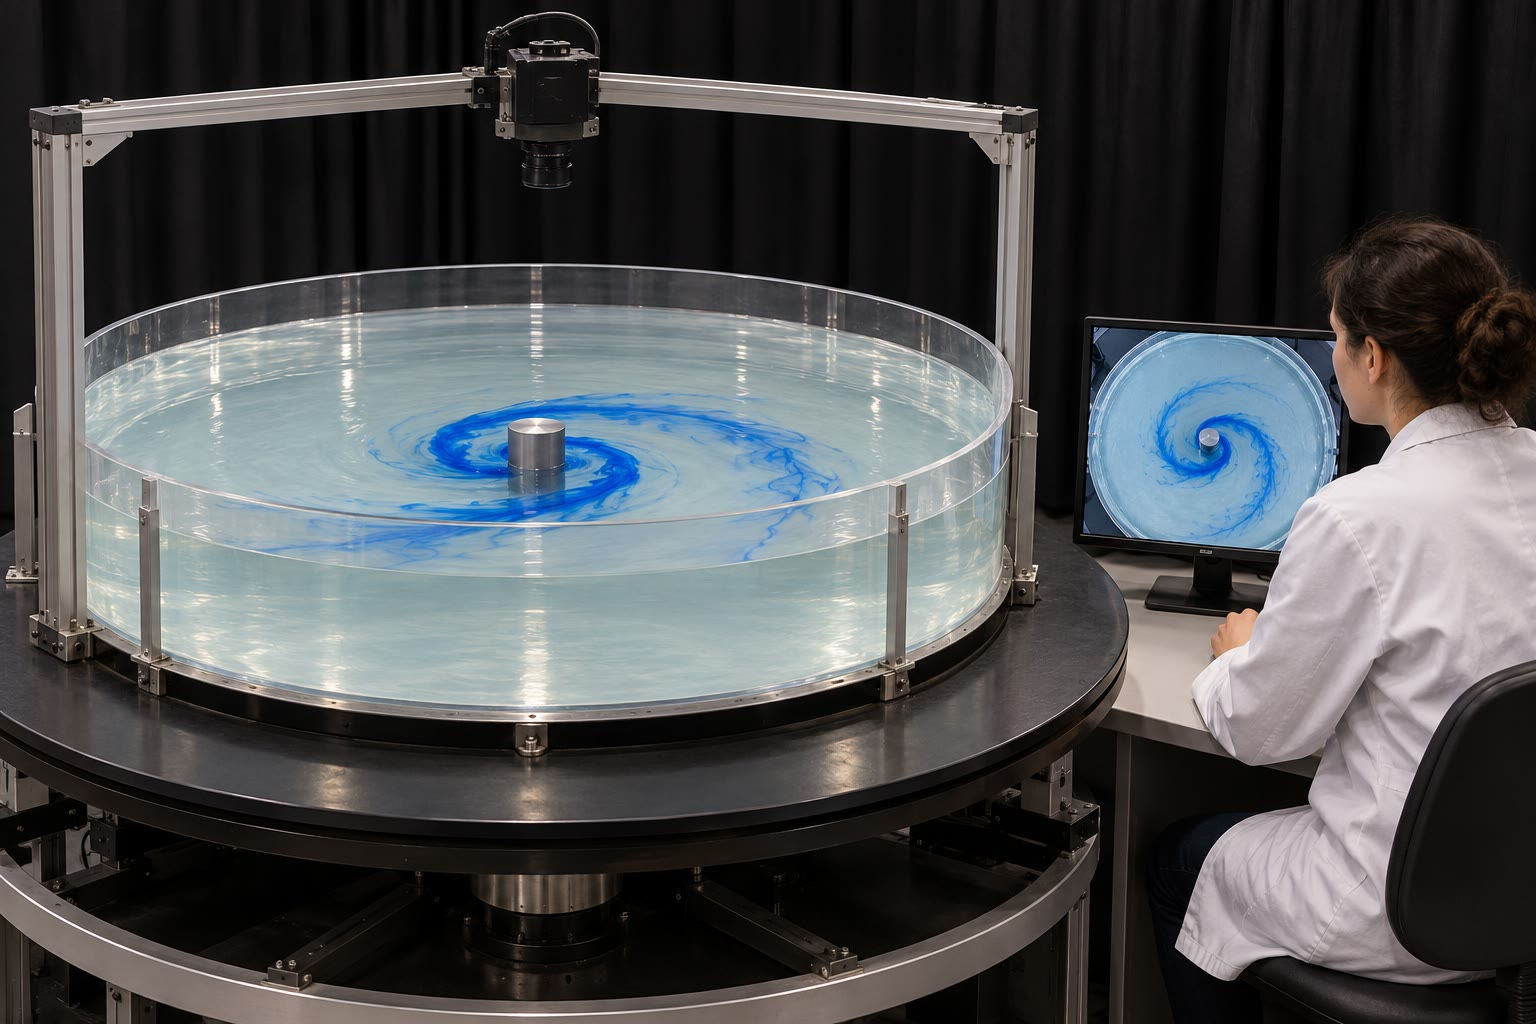
\includegraphics[width=\linewidth]{images/book5/ai/b3-rotating-tank.jpg}

{\scriptsize Un tanque en rotación: colorante en espiral alrededor de un cilindro, filmado por una
cámara que gira con la mesa (ilustración generada por IA).}
\end{minipage}
\end{inthelab}

\section{Ejercicios}

\begin{exercise}[$\star$]\label{exo:b3:gfd-foundations:1}
Tómese $\Omega = \qty{7.292115e-5}{rad/s}$. (a)~Calcúlense el parámetro de Coriolis y el
período inercial a \ang{30}, \ang{45} y \ang{60} N.
(b)~Calcúlese el radio del círculo inercial de una corriente de
\qty{0.20}{m/s} a las mismas latitudes. (c)~Compárese el período inercial a
\ang{30} con el día sidéreo, \qty{23.9345}{h}.
\end{exercise}

\begin{exercise}[$\star$]\label{exo:b3:gfd-foundations:2}
A \ang{45} N, calcúlese el \omterm{def:b3:gfd-foundations:numbers}{número de Rossby} de un torbellino de polvo (\qty{10}{m/s},
\qty{10}{m}), una brisa marina (\qty{5}{m/s}, \qty{20}{km}), una depresión
(\qty{15}{m/s}, \qty{1000}{km}) y un giro oceánico (\qty{0.05}{m/s},
\qty{2000}{km}). ¿Cuáles de ellos están cerca del equilibrio geostrófico?
\end{exercise}

\begin{exercise}[$\star$]\label{exo:b3:gfd-foundations:3}
A \ang{45} N, la temperatura media de la troposfera, \qty{250}{K}, disminuye
hacia el norte \qty{5}{K} por cada \qty{1000}{km}. Utilícese el primer término del
\omterm{thm:b3:gfd-foundations:thermal-wind}{viento térmico} en altura, calcúlese el cizallamiento vertical del viento del oeste y el
aumento del viento en \qty{10}{km}.
\end{exercise}

\begin{exercise}[$\star$]\label{exo:b3:gfd-foundations:4}
La estabilidad $E = -(1/\rho)\,\mathrm d\rho_\theta/\mathrm dz$ del kilómetro superior
del océano se encuentra entre \num{50e-8} y \qty{1000e-8}{m^{-1}};
en las fosas profundas vale \qty{e-8}{m^{-1}}. Calcúlense $N = \sqrt{gE}$, el período
de la oscilación de flotabilidad y $N$ en ciclos por hora para estos
tres valores.
\end{exercise}

\begin{exercise}[$\star\star$]\label{exo:b3:gfd-foundations:5}
Un sistema meteorológico tiene $U = \qty{10}{m/s}$, $L = \qty{1000}{km}$, $H =
\qty{10}{km}$, a \ang{45} N. (a)~Estímese su velocidad vertical y su aceleración
vertical, y compárese esta última con $g$ y con el gradiente vertical de la
perturbación de presión, $fUL/H$. (b)~Calcúlese el término de Coriolis despreciado
$\tilde fu$ y compárese con $g$.
\end{exercise}

\begin{exercise}[$\star\star$]\label{exo:b3:gfd-foundations:6}
Tómese $f = \qty{e-4}{s^{-1}}$ e isobaras circulares de radio
\qty{300}{km}. (a)~El gradiente de presión alrededor de una borrasca da $V_g =
\qty{20}{m/s}$: calcúlese el \omterm{def:b3:gfd-foundations:gradient}{viento del gradiente}. (b)~Alrededor de un anticiclón,
$V_g = \qty{5}{m/s}$: calcúlese el \omterm{def:b3:gfd-foundations:gradient}{viento del gradiente}. (c)~¿Cuál es el mayor
$V_g$ posible alrededor del anticiclón, y entonces el viento?
\end{exercise}

\begin{exercise}[$\star\star$]\label{exo:b3:gfd-foundations:7}
Un tanque de \qty{20}{cm} de profundidad gira una vez cada \qty{6}{s}; su agua tiene $\nu =
\qty{e-6}{m^2/s}$. (a)~Calcúlese $f = 2\Omega$, después el \omterm{def:b3:gfd-foundations:numbers}{número de Rossby} de un
flujo de \qty{1}{cm/s} que pasa un cilindro de \qty{5}{cm} de diámetro, y el \omterm{def:b3:gfd-foundations:numbers}{número de
Ekman} del tanque. ¿Se formará una \omterm{thm:b3:gfd-foundations:taylor-proudman}{columna de Taylor}? (b)~La teoría da un tiempo de spin-up
$H/\sqrt{\nu\Omega}$: calcúlese en minutos y en vueltas de la mesa.
\end{exercise}

\begin{exercise}[$\star\star$]\label{exo:b3:gfd-foundations:8}
En la media zonal de enero de 1991--2020 el viento del oeste vale \qty{4.27}{m/s}
a \qty{850}{hPa} y \qty{40.39}{m/s} a \qty{250}{hPa} a \ang{30} N,
\qty{5.99}{m/s} y \qty{23.17}{m/s} a \ang{45} N. Con $R =
\qty{286.9}{J.kg^{-1}.K^{-1}}$, calcúlese el gradiente meridional de la temperatura
media de la capa a ambas latitudes, y explíquese por qué la corriente en chorro es
más intensa a \ang{30} N.
\end{exercise}

\begin{exercise}[$\star\star$]\label{exo:b3:gfd-foundations:9}
(a)~Calcúlese el \omterm{def:b3:gfd-foundations:rossby-radius}{radio de deformación de Rossby} de la troposfera ($N =
\qty{0.0113}{s^{-1}}$, $H = \qty{11}{km}$, \ang{45} N) y del océano superior
($N = \qty{0.00357}{s^{-1}}$, $H = \qty{1000}{m}$, \ang{40.5} N).
(b)~Con $a = \qty{6371}{km}$, calcúlese $\beta$ a ambas latitudes y el cambio relativo
$\beta L_R/f$ del parámetro de Coriolis a lo largo de cada radio.
\end{exercise}

\begin{exercise}[$\star\star\star$]\label{exo:b3:gfd-foundations:10}
Una partícula de agua de la superficie del océano, que se mueve a velocidad $U$, se frena por
una fricción lineal: $\mathrm du/\mathrm dt = fv - ru$, $\mathrm dv/\mathrm dt = -fu -
rv$. (a)~Resuélvase con $w = u + \mathrm iv$ y descríbase la trayectoria. (b)~La
partícula es arrastrada además por una corriente estacionaria $u_0$ hacia el este: dese su
posición. (c)~A \ang{45} N, con $U = \qty{0.2}{m/s}$, $r^{-1} =
\num{4}~\text{días}$ y $u_0 = \qty{0.05}{m/s}$, dese su velocidad relativa a la corriente
tras cuatro días y la distancia que ha derivado.
\end{exercise}

\begin{exercise}[$\star\star\star$]\label{exo:b3:gfd-foundations:11}
A través de un frente oceánico a \ang{40} N, la densidad del agua aumenta hacia el norte
\qty{1}{kg/m^3} en \qty{100}{km}, en los
\qty{1000}{m} superiores; por debajo, el agua es uniforme y está en reposo. Con $\rho_0 =
\qty{1025}{kg/m^3}$, calcúlense el cizallamiento vertical de la corriente y la
corriente en la superficie. ¿En qué dirección fluye?
\end{exercise}

\begin{exercise}[$\star\star\star$]\label{exo:b3:gfd-foundations:12}
La columna media anual en \ang{40.5} N, \ang{30.5} O presenta
densidades potenciales $\sigma_\theta = \rho_\theta - \qty{1000}{kg/m^3}$ de 26.029 en
la superficie, 26.697 a \qty{100}{m}, 27.079 a \qty{500}{m} y 27.628 a
\qty{1000}{m}. (a)~Calcúlese $N$ en cada una de las tres capas, en
\unit{s^{-1}} y en ciclos por hora. (b)~¿Qué capa es la más estable,
y por qué? (c)~Compárense los valores con el intervalo del océano superior
recogido en el \cref{exo:b3:gfd-foundations:4}.
\end{exercise}
% ledger: geod5:grs80-defining, earth:Trot, stewart:stability, data:b5-ncep-uwnd, data:b5-woa23-atlantic, earth:Rmean

\section{Problema: vientos sobre la estepa de Orrin}

\begin{problem}[{Problema de fin de semana --- la rotación, la estratificación y
los vientos de una llanura inventada a \ang{48} N}]
\label{pb:b3:gfd-foundations:1}
La estepa de Orrin es una llanura plana a \ang{48} N con un lago, el lago Orrin,
de \qty{12}{km} de anchura, y un pequeño laboratorio con un tanque giratorio. Tómense
$\Omega = \qty{7.292115e-5}{rad/s}$, $g = \qty{9.81}{m/s^2}$, $R =
\qty{286.9}{J.kg^{-1}.K^{-1}}$ y $c_p = \qty{1004}{J.kg^{-1}.K^{-1}}$.
Todos los valores de la estepa, de su lago y de sus vientos son inventados.

\medskip\noindent\textbf{Parte I --- ¿Importa la rotación?}
\begin{enumerate}
\item Calcúlense el parámetro de Coriolis y el periodo inercial en Orrin.
\item Calcúlese el \omterm{def:b3:gfd-foundations:numbers}{número de Rossby} de cinco flujos: agua que desagua de una bañera
  (\qty{0.1}{m/s} sobre \qty{0.3}{m}); el tanque del laboratorio, que gira
  una vez cada \qty{10}{s} (con $f = 2\Omega_{\text{tanque}}$; \qty{5}{mm/s}
  sobre \qty{0.2}{m}); la brisa de la tarde desde el lago (\qty{5}{m/s},
  \qty{20}{km}); una depresión (\qty{15}{m/s}, \qty{1000}{km}); el giro de una
  cuenca oceánica a la misma latitud (\qty{0.05}{m/s}, \qty{2000}{km}).
\item ¿Cuáles de estos flujos sienten la rotación que los impulsa, y cuáles están
  próximos al equilibrio geostrófico?
\item Calcúlese el \omterm{def:b3:gfd-foundations:numbers}{número de Ekman} del tanque (\qty{0.2}{m} de profundidad, $\nu =
  \qty{e-6}{m^2/s}$), de la depresión (viscosidad de remolino \qty{10}{m^2/s},
  profundidad \qty{10}{km}) y del giro (viscosidad de remolino \qty{e-3}{m^2/s},
  profundidad \qty{1000}{m}).
\item La capa de Ekman tiene el espesor $\delta = \sqrt{2\nu/f}$. Demuéstrese que
  $\delta/H = \sqrt{2\,\mathrm{Ek}}$ y calcúlese $\delta$ para el tanque y para
  el aire de la estepa.
\item ¿Qué indican estos números sobre dónde importa la fricción?
\end{enumerate}

\medskip\noindent\textbf{Parte II --- El viento en superficie.}
\begin{enumerate}[resume]
\item En superficie la presión es \qty{1012.9}{hPa} y la temperatura
  \qty{288.1}{K}. Calcúlese la densidad del aire.
\item La presión a nivel del mar disminuye hacia el norte en \qty{4}{hPa} por
  \qty{300}{km}. Calcúlese el viento geostrófico e indíquese su dirección.
\item El mismo gradiente rodea una depresión cuyas isobaras tienen un radio
  de \qty{600}{km}. Calcúlese el \omterm{def:b3:gfd-foundations:numbers}{número de Rossby} de las isobaras y el
  \omterm{def:b3:gfd-foundations:gradient}{viento del gradiente}.
\item El mismo gradiente rodea un anticiclón del mismo radio.
  Calcúlese el \omterm{def:b3:gfd-foundations:gradient}{viento del gradiente} y el mayor gradiente de presión, en
  \unit{hPa} por \qty{300}{km}, que puede mantener el anticiclón.
\end{enumerate}

\medskip\noindent\textbf{Parte III --- Estratificación.}
\begin{enumerate}[resume]
\item La temperatura de la troposfera disminuye a razón de \qty{6.49}{K/km}.
  Calcúlese el gradiente adiabático seco $g/c_p$, y $N$ y el periodo de
  la oscilación de flotabilidad a \qty{5}{km}, donde la temperatura es
  \qty{255.7}{K}.
\item Por encima de \qty{11}{km} el aire es isotermo a \qty{216.6}{K}. Demuéstrese que
  $N^2 = g^2/(c_pT)$ allí, y calcúlense $N$ y su razón con el valor de
  la pregunta~11.
\item Calcúlese el \omterm{def:b3:gfd-foundations:rossby-radius}{radio de deformación de Rossby} de la troposfera de Orrin, con el $N$ de
  la pregunta~11 y $H = \qty{10}{km}$, y compárese con el tamaño de la
  depresión de la Parte~I.
\item En verano, los \qty{20}{m} superiores del lago Orrin son
  \qty{1.5}{kg/m^3} más ligeros que el agua profunda ($\rho_0 = \qty{1000}{kg/m^3}$). Calcúlense
  la gravedad reducida $g' = g\,\Delta\rho/\rho_0$, la velocidad $\sqrt{g'h}$ de
  las ondas internas lentas de la capa superior, y el \omterm{def:b3:gfd-foundations:rossby-radius}{radio de deformación de Rossby}
  $\sqrt{g'h}/f$.
\item ¿Condicionará la rotación de la Tierra los movimientos internos del lago?
\end{enumerate}

\medskip\noindent\textbf{Parte IV --- El viento térmico.}
\begin{enumerate}[resume]
\item Dos estaciones de radiosondeo distan \qty{600}{km} entre sí en el mismo
  meridiano. La temperatura media de la capa desde el suelo,
  \qty{1013}{hPa}, hasta \qty{265}{hPa}, de unos \qty{10}{km}, es \qty{253.0}{K}
  en la estación meridional y \qty{249.4}{K} en la septentrional. Calcúlese el
  gradiente meridional de temperatura en \unit{K} por \qty{1000}{km}.
\item El espesor de una capa entre dos presiones es $\Delta z = (R\bar
  T/g)\ln(p_b/p_t)$. Calcúlese en ambas estaciones, y la pendiente de la
  superficie de \qty{265}{hPa} respecto a la del nivel del suelo.
\item Dedúzcase el aumento del viento geostrófico desde el suelo hasta
  \qty{265}{hPa}, a partir de esa pendiente.
\item Calcúlese el mismo aumento con el teorema del \omterm{thm:b3:gfd-foundations:thermal-wind}{viento térmico} en presión.
\item ¿Es el aire de la estepa \omterm{def:b3:gfd-foundations:baroclinic}{barotrópico} o \omterm{def:b3:gfd-foundations:baroclinic}{baroclínico}? ¿Cuál sería el viento
  a \qty{265}{hPa} si fuera \omterm{def:b3:gfd-foundations:baroclinic}{barotrópico}?
\item Calcúlese el aumento a partir del primer término del \omterm{thm:b3:gfd-foundations:thermal-wind}{viento térmico} en
  altura, con la temperatura media de la troposfera estándar entre 0
  y \qty{10}{km}, \qty{255.7}{K}, y compárese.
\item Calcúlese el viento a \qty{541}{hPa}, de unos \qty{5}{km}, suponiendo que el
  gradiente de temperatura es el mismo en todos los niveles.
\item El número de Richardson $N^2/(\partial u/\partial z)^2$ debe caer por debajo de
  0.25 para que la cizalladura genere turbulencia. Calcúlese para la troposfera de
  Orrin.
\item En enero la media zonal del viento del oeste a \qty{250}{hPa} es \qty{23.2}{m/s}
  a \ang{45} N y \qty{40.4}{m/s} a \ang{30} N. Compárese con el viento de
  Orrin, y explíquese por qué un viento local puede superar a la media zonal.
\item Indíquese el viento geostrófico a \qty{10}{km} sobre la estepa de Orrin.
\end{enumerate}
\end{problem}
% ledger: geod5:grs80-defining, stewart:stability, data:b5-ncep-uwnd, nasa:grc-atmos
